% F049: native TikZ/PGFPlots, computed from the stated mathematical model.
\begin{center}
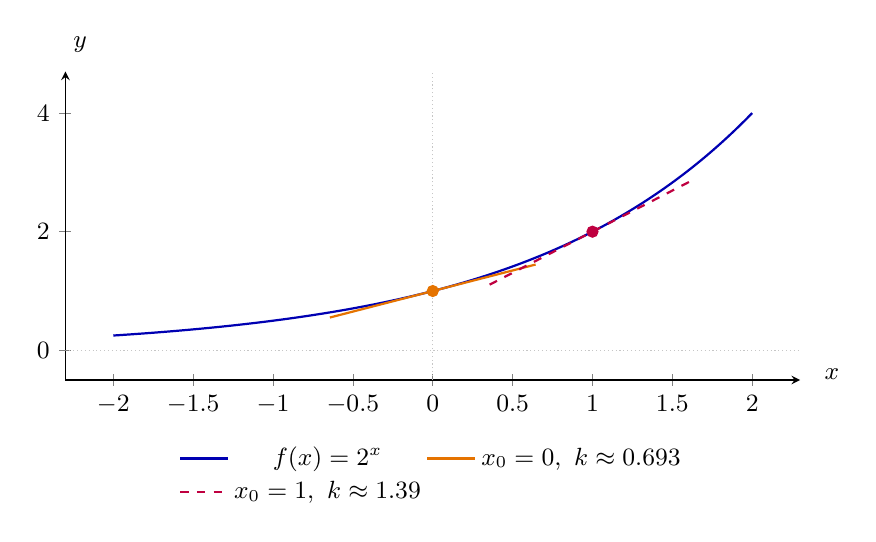
\begin{tikzpicture}[font=\small,>=stealth]
\begin{axis}[width=.90\linewidth,height=5.5cm,xmin=-2.3,xmax=2.3,ymin=-0.5,ymax=4.7,
axis lines=left,xlabel={$x$},ylabel={$y$},font=\small,
xlabel style={at={(axis description cs:1.02,.02)},anchor=west},
ylabel style={rotate=-90,at={(axis description cs:.02,1.03)},anchor=south},
legend style={at={(axis description cs:.5,-.18)},anchor=north,draw=none,fill=none,font=\small,legend columns=2},
unbounded coords=jump,clip=true,]
\addplot[gray!45,thin,densely dotted,forget plot] coordinates {(-2.3,0) (2.3,0)};
\addplot[gray!45,thin,densely dotted,forget plot] coordinates {(0,-0.5) (0,4.7)};
\addplot[blue!70!black,thick] coordinates {(-2,0.25) (-1.9777778,0.25388063) (-1.9555556,0.25782149) (-1.9333333,0.26182353) (-1.9111111,0.26588769) (-1.8888889,0.27001493) (-1.8666667,0.27420624) (-1.8444444,0.27846261) (-1.8222222,0.28278505) (-1.8,0.28717459) (-1.7777778,0.29163226) (-1.7555556,0.29615913) (-1.7333333,0.30075626) (-1.7111111,0.30542475) (-1.6888889,0.31016571) (-1.6666667,0.31498026) (-1.6444444,0.31986955) (-1.6222222,0.32483473) (-1.6,0.32987698) (-1.5777778,0.3349975) (-1.5555556,0.3401975) (-1.5333333,0.34547822) (-1.5111111,0.35084091) (-1.4888889,0.35628684) (-1.4666667,0.36181731) (-1.4444444,0.36743362) (-1.4222222,0.37313712) (-1.4,0.37892914) (-1.3777778,0.38481107) (-1.3555556,0.39078431) (-1.3333333,0.39685026) (-1.3111111,0.40301038) (-1.2888889,0.40926611) (-1.2666667,0.41561895) (-1.2444444,0.4220704) (-1.2222222,0.42862199) (-1.2,0.43527528) (-1.1777778,0.44203185) (-1.1555556,0.44889329) (-1.1333333,0.45586124) (-1.1111111,0.46293736) (-1.0888889,0.47012331) (-1.0666667,0.4774208) (-1.0444444,0.48483157) (-1.0222222,0.49235738) (-1,0.5) (-0.97777778,0.50776126) (-0.95555556,0.51564299) (-0.93333333,0.52364706) (-0.91111111,0.53177538) (-0.88888889,0.54002987) (-0.86666667,0.54841249) (-0.84444444,0.55692523) (-0.82222222,0.56557011) (-0.8,0.57434918) (-0.77777778,0.58326452) (-0.75555556,0.59231825) (-0.73333333,0.60151252) (-0.71111111,0.6108495) (-0.68888889,0.62033142) (-0.66666667,0.62996052) (-0.64444444,0.6397391) (-0.62222222,0.64966945) (-0.6,0.65975396) (-0.57777778,0.66999499) (-0.55555556,0.680395) (-0.53333333,0.69095644) (-0.51111111,0.70168182) (-0.48888889,0.71257368) (-0.46666667,0.72363462) (-0.44444444,0.73486725) (-0.42222222,0.74627423) (-0.4,0.75785828) (-0.37777778,0.76962215) (-0.35555556,0.78156862) (-0.33333333,0.79370053) (-0.31111111,0.80602075) (-0.28888889,0.81853222) (-0.26666667,0.8312379) (-0.24444444,0.8441408) (-0.22222222,0.85724398) (-0.2,0.87055056) (-0.17777778,0.8840637) (-0.15555556,0.89778659) (-0.13333333,0.91172249) (-0.11111111,0.92587471) (-0.088888889,0.94024661) (-0.066666667,0.9548416) (-0.044444444,0.96966314) (-0.022222222,0.98471475) (0,1) (0.022222222,1.0155225) (0.044444444,1.031286) (0.066666667,1.0472941) (0.088888889,1.0635508) (0.11111111,1.0800597) (0.13333333,1.096825) (0.15555556,1.1138505) (0.17777778,1.1311402) (0.2,1.1486984) (0.22222222,1.166529) (0.24444444,1.1846365) (0.26666667,1.203025) (0.28888889,1.221699) (0.31111111,1.2406628) (0.33333333,1.259921) (0.35555556,1.2794782) (0.37777778,1.2993389) (0.4,1.3195079) (0.42222222,1.33999) (0.44444444,1.36079) (0.46666667,1.3819129) (0.48888889,1.4033636) (0.51111111,1.4251474) (0.53333333,1.4472692) (0.55555556,1.4697345) (0.57777778,1.4925485) (0.6,1.5157166) (0.62222222,1.5392443) (0.64444444,1.5631372) (0.66666667,1.5874011) (0.68888889,1.6120415) (0.71111111,1.6370644) (0.73333333,1.6624758) (0.75555556,1.6882816) (0.77777778,1.714488) (0.8,1.7411011) (0.82222222,1.7681274) (0.84444444,1.7955732) (0.86666667,1.823445) (0.88888889,1.8517494) (0.91111111,1.8804932) (0.93333333,1.9096832) (0.95555556,1.9393263) (0.97777778,1.9694295) (1,2) (1.0222222,2.031045) (1.0444444,2.0625719) (1.0666667,2.0945882) (1.0888889,2.1271015) (1.1111111,2.1601195) (1.1333333,2.19365) (1.1555556,2.2277009) (1.1777778,2.2622804) (1.2,2.2973967) (1.2222222,2.3330581) (1.2444444,2.369273) (1.2666667,2.4060501) (1.2888889,2.443398) (1.3111111,2.4813257) (1.3333333,2.5198421) (1.3555556,2.5589564) (1.3777778,2.5986778) (1.4,2.6390158) (1.4222222,2.67998) (1.4444444,2.72158) (1.4666667,2.7638258) (1.4888889,2.8067273) (1.5111111,2.8502947) (1.5333333,2.8945385) (1.5555556,2.939469) (1.5777778,2.9850969) (1.6,3.0314331) (1.6222222,3.0784886) (1.6444444,3.1262745) (1.6666667,3.1748021) (1.6888889,3.224083) (1.7111111,3.2741289) (1.7333333,3.3249516) (1.7555556,3.3765632) (1.7777778,3.4289759) (1.8,3.4822023) (1.8222222,3.5362548) (1.8444444,3.5911463) (1.8666667,3.64689) (1.8888889,3.7034988) (1.9111111,3.7609865) (1.9333333,3.8193664) (1.9555556,3.8786526) (1.9777778,3.938859) (2,4)};
\addlegendentry{$f(x)=2^x$}
\addplot[orange!90!black,thick] coordinates {(-0.644,0.55361322) (0.644,1.4463868)};
\addlegendentry{$x_0=0,\ k\approx0.693$}
\addplot[only marks,mark=*,orange!90!black,forget plot] coordinates {(0,1)};
\addplot[purple,thick,dashed] coordinates {(0.356,1.1072264) (1.644,2.8927736)};
\addlegendentry{$x_0=1,\ k\approx1.39$}
\addplot[only marks,mark=*,purple,forget plot] coordinates {(1,2)};

\end{axis}
\end{tikzpicture}
\par\smallskip{\small $a>0$；图中取 $a=2$，一般底数的正负变化见易错一。}
\end{center}
